% Plantilla latex para protocolo de tesis de posgrado en la 
% Facultad de Ingeniería, Universidad Autónoma de Querétaro
%
% @author {Gerardo Hernández-Nava, Enrique Mena-Camilo, Sheila Leyva-López}
% @email {gerardohn.uam@gmail.com, enriquemece97@gmail.com, sheileyva29@gmail.com}
% @year 2022
% @version 1.0
% @license CC-BY-NC
%
% Se agradecen sus comentarios, contribuciones, 
% reporte de bugs y la difusión de esta plantilla


\documentclass[12pt, letterpaper, spanish, twoside]{article}
\AddToHook{cmd/section/before}{\clearpage}
\usepackage{./common/UAQ}

\usepackage{xcolor}
\usepackage{emptypage}
\setlength{\cftsecnumwidth}{3em} %Se cambia el espacio entre el item y el nombre de la seccion
\setlength{\cftsubsecnumwidth}{3em}
\setlength{\cftsubsecindent}{3em}
\setlength{\cftsubsubsecindent}{6em}

\usepackage{threeparttablex}
\usepackage{adjustbox}
\usepackage{caption}
\usepackage{subcaption}

\graphicspath{{./figures/}, {../figures}}

\usepackage{tabulary}
\newcolumntype{K}[1]{>{\centering\arraybackslash}p{#1}}

\usepackage{minted}
\usepackage[section]{placeins}
\usepackage{multirow}
\usepackage{booktabs}
\usepackage{algorithm}
\usepackage{algpseudocode}
\makeatletter
\renewcommand{\ALG@name}{Algoritmo}
\makeatother

\begin{document}
\renewcommand{\tablename}{Tabla}

% Fondo de portada
\backgroundsetup{
	scale = 1,
	angle = 0,
	opacity = 1,
	contents = {
		
\includegraphics[width=\paperwidth]{CoverBackground.pdf}
	}
}

\begin{titlepage}

\vspace*{10cm}
{\huge \bfseries \textcolor{RojoUAQ}{Algoritmos Metaheurísticos: \\ Examen 2. Algoritmo Genético: Optimización de precio de productos lacteos.}}

\vspace*{1cm}

\begin{center}
	\noindent
	\begin{minipage}{0.4\textwidth}
	\begin{flushleft} \large
	\end{flushleft}
	\end{minipage}	
	\begin{minipage}{0.5\textwidth}
	\begin{flushright} \large
	\emph{Alumno:} \\
	Ing. Enrique Mena Camilo \\[1.5cm]
	\emph{Profesor:} \\
	Dr. Marco Antonio Aceves Fernández
	\end{flushright}
	\end{minipage}
	\vfill
	{\large Diciembre 2023}
\end{center}
\end{titlepage}


\backgroundsetup{
	scale = 1,
	angle = 0,
	opacity = 1,
	contents = {
\includegraphics[width=\paperwidth]{BodyBackground.pdf}}}

\pagenumbering{Roman}
\tableofcontents
\newpage

\pagenumbering{arabic}

\section{Objetivos}
El objetivo de esta práctica consiste en encontrar soluciones a un problema industrial, la producción de papel en una fábrica de papel. Esta solución deberá permitir la modificación de parámetros previo a su ejecución, así como contemplar diversos tipos de papel y grosores. La solución deberá implementarse mediante algoritmos genéticos.


\section{Introducción}
Sea una planta de producción continua de papel. La misma consiste de un mesa formadora en donde se pone la pasta de papel (fibras celulósicas más otros componentes). La mesa formadora alimenta una serie de rodillos calentados a alta temperatura que secan y comprimen la pasta, generando, de esa manera, el papel. Se pueden producir diferentes colores y calidades de papel. Para cada par de estos corresponden capacidades máximas de producción. (El papel se mide por el gramaje que es el peso en gramos de un metro cuadrado del mismo). Cuanto más alto es el gramaje, menos es la producción horaria, debido a las limitaciones impuestas por la máxima capacidad de trabajo de la máquina. Cuanto más gramaje mayor es el flujo de masa y por lo tanto mayor es la necesidad de potencia para generar el suficiente calor para secarlo y la suficiente presión para laminarlo y llevarlo al espesor deseado. A menores gramajes (papel más fino) la limitación está dada por la resistencia a la rotura del papel, ya que el aumento de la capacidad de producción requeriría velocidades que harían que el papel se rompiera obligando a parar la planta y reiniciar el proceso de producción.

\section{Marco teórico}
\subsection{Roulette Selection}
El mecanismo de selección de ruleta, es una técnica popularmente usada en algoritmos genéticos para seleccionar posibles soluciones de acuerdo a su aptitud. La idea es dar a cada individuo una probabilidad de ser seleccionado que sea proporcional a su aptitud, de tal manera que los individuos con mayor aptitud tengan una mayor probabilidad de ser elegidos, pero aún permitiendo que los individuos con menor aptitud tengan alguna posibilidad.

En términos generales, este método consta de los siguientes pasos:

\begin{enumerate}
	\item Cálculo de Aptitudes: En primer lugar, se calcula la aptitud de cada individuo en la población.
	\item Suma de Aptitudes: Se suman todas las aptitudes para obtener una aptitud total de la población.
	\item Cálculo de Probabilidades: Se determina la probabilidad de selección de cada individuo dividiendo su aptitud por la aptitud total de la población.
	\item Selección: Se genera un número aleatorio entre 0 y 1. Luego, se selecciona el individuo cuya probabilidad acumulada incluye este número aleatorio. En otras palabras, imaginamos que giramos una ruleta donde cada segmento corresponde a un individuo, y el tamaño de cada segmento es proporcional a la aptitud del individuo.
\end{enumerate}

Una representación gráfica de este mecanismo se puede observar en la Figura \ref{fig:RS}.

\begin{figure}[htbp]
	\centering
	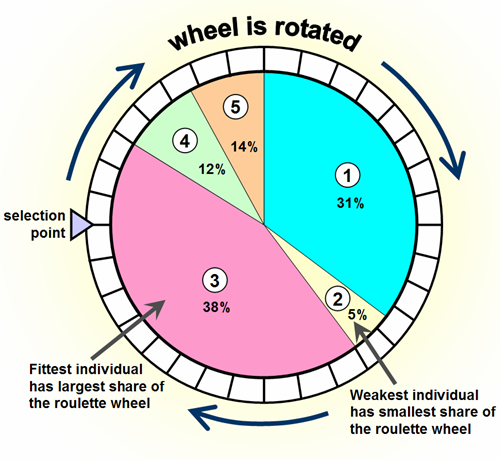
\includegraphics[width=0.4\textwidth]{roulette_selection}
	\caption{Diagrama de funcionamiento de selección por ruleta.}
	\label{fig:RS}
\end{figure}


\subsection{Two Point Crossover}
La cruza de dos puntos (two point crossover, en inglés) es un método de recombinación comúnmente utilizado en algoritmos genéticos que permite la combinación de características de dos padres para generar una descendencia. Este método permite generar combinaciones de características de ambos padres para explorar y buscar mejores soluciones. En terminos generales, este método consta de los siguientes pasos:

\begin{enumerate}
	\item Definición de Puntos de Corte: Se seleccionan dos puntos de corte en la representación de los padres. Estos puntos dividen a los padres en tres segmentos: el segmento antes del primer punto de corte, el segmento entre los dos puntos de corte y el segmento después del segundo punto de corte.
	\item Creación de Descendencia: La descendencia se crea intercambiando los segmentos intermedios (el segmento entre los dos puntos de corte) de los dos padres. El resultado es un nuevo individuo que combina partes de ambos padres.
\end{enumerate}

\begin{figure}[htbp]
	\centering
	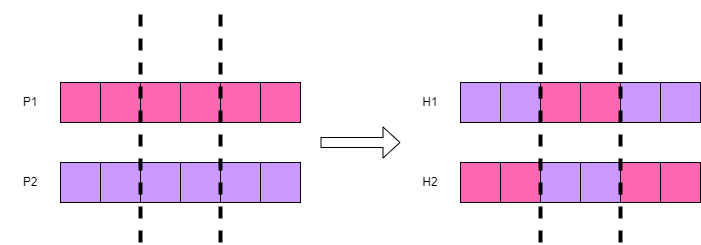
\includegraphics[width=0.8\textwidth]{crossover_two}
	\caption{Mecanismo de cruza de dos puntos.}
	\label{fig: cross_two}
\end{figure}


\subsection{Scramble Mutation}
La mutación por mezcla (scramble mutation, en inglés) es un proceso que introduce pequeños cambios aleatorios en los individuos de una población con el objetivo de aumentar la diversidad genética y explorar nuevas soluciones en el espacio de búsqueda. Dicho proceso se caracteriza por los siguientes pasos:

\begin{enumerate}
	\item Selección de un subconjunto de genes: Se elige un subconjunto aleatorio de genes en la representación del individuo. Los genes seleccionados formarán parte del proceso de mutación.
	\item Mezcla de genes: Los genes seleccionados se reordenan de manera aleatoria entre sí. Este reordenamiento aleatorio puede ser realizado de diferentes maneras, como permutando los valores de los genes dentro del subconjunto o cambiando su posición en la secuencia.
\end{enumerate}

Podemos observar una representación gráfica de este mecanismo en la Figura \ref{fig:scrM}.

\begin{figure}[htbp]
	\centering
	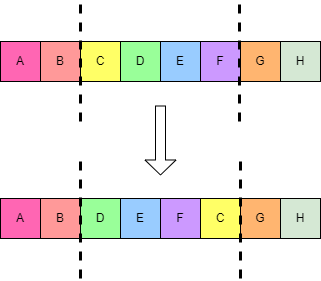
\includegraphics[width=0.4\textwidth]{scramble_mutation}
	\caption{Diagrama de funcionamiento de scramble mutation.}
	\label{fig:scrM}
\end{figure}


\subsection{Competencia genética}
El concepto de competencia genética se asemeja a la lucha por la supervivencia en la naturaleza, donde los individuos más aptos tienen una mayor probabilidad de sobrevivir y reproducirse, transmitiendo así sus genes a la siguiente generación. La idea principal detrás de la competencia genética en algoritmos evolutivos es simular este proceso de selección natural para buscar soluciones óptimas o mejores en un espacio de búsqueda.

En este proceso se toma a todos los padres y a todos los hijos, se ordenan de mayor a menor aptitud, y solamente se permitirá que pasen a la siguiente generación aquellos que presentan mejor aptitud, sin importar sin son padres o hijos.


\section{Materiales y métodos}
\subsection{Análisis exploratorio de datos}
Se realizó un análisis exploratorio de los datos, el cuál permitió identificar valores de estadística descriptiva de los precios de cada uno de los productos. Para este análisis solamente se tomó en cuenta los precios de los últimos 6 años.

Este proceso adicionalmente implementó un proceso de limpieza de datos, donde se logró estandarizar los diferentes formatos de fecha presentes, así como extraer información como año, mes y trimestre del año.

Teniendo los datos preparados se procedió a obtener gráficas de la distribución del precio de cada producto a lo largo de los diferentes años analizados, así como gráficas que permiten realizar un análisis del precio de los productos en cada trimestre y cómo fue su comportamiento a lo largo de todos los años analizados.


\subsection{Funciones de aptitud}
Partiendo del modelo básico de optimización de precio, se procedió a generar datos sintéticos para el inventario de cada uno de los productos a lo largo del periodo analizado. Este proceso de generación de datos sintéticos se realizó con las siguientes reglas:

\begin{itemize}
	\item Valor máximo: $10,000$ toneladas.
	\item Valor mínimo: $2,000$ toneladas.
	\item Valor promedio: $5,000$ toneladas.
	\item Desviación estándar:
	\begin{itemize}
		\item Lactosa: $2,000$ toneladas.
		\item Suero: $1,500$ toneladas.
	\end{itemize}
\end{itemize}

Teniendo los datos sintéticos de inventario, se insertaron de forma aleatoria a nuestro conjunto de datos para simular la demanda del producto ante cada precio, donde se tomó la asunción de una venta completa, es decir, la demanda del producto fue la misma que le inventario.

Teniendo las consideraciones anteriores, se procedió a obtener un modelo lineal que se ajuste a la variación de la demanda según el precio. Estos modelos lineales siguen la forma de la función de demanda (Ecuación \ref{eq:demand}).

Una vez estimada la función de demanda para cada producto de interés, se procedió a implementar la función de ganancia (Ecuación \ref{eq:revenue}) con una ligera variación. Considerando que se tienen 2 tipos de cliente (un cliente estándar que compra poco producto y suele tener un precio estándar; un cliente premium que compra grandes cantidades de producto y suele tener un descuento al precio estándar), se procedió a modificar la función de ganancia para que esta considere el precio mas un 10\%, al realizar esta modificación incrementamos el precio para el cliente estándar, permitiendo también que al cliente premium le apliquemos un descuento y no perdamos ganancias. Tomando esas consideraciones finales, el modelo básico de optimización de precio se estableció como la Ecuación\ref{eq:price2}

\begin{equation}\label{eq:price2}
	R(p)= (p+0.10*p)(a-b(p+0.10*p))
\end{equation}


\subsection{Algoritmo genético}
Para esta práctica se desarrolló un algoritmo genético que se apega al proceso mostrado en la Figura \ref{fig:AG}.

\begin{figure}[htbp]
	\centering
	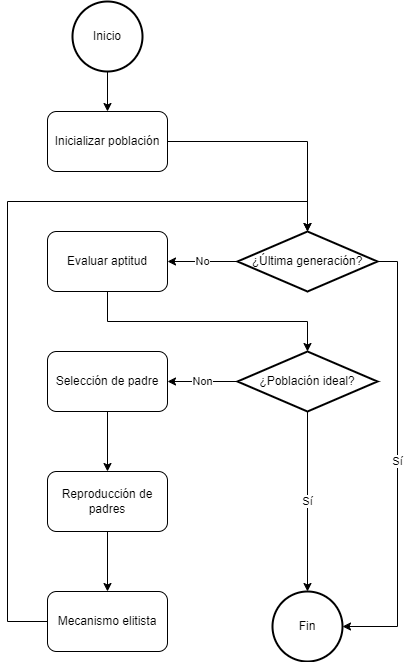
\includegraphics[width=0.35\textwidth]{algoritmo_genetico_proceso}
	\caption{Diagrama de flujo del algoritmo genético implementado.}
	\label{fig:AG}
\end{figure}

Para llevar a cabo dicho proceso, se optó por utilizar el lenguaje de programación Python, donde se diseñaron métodos genéricos para realizar los procesos de generación de población, evaluación de aptitud, selección de individuos, reproducción de individuos, mutación y mecanismos elitistas.


\subsection{Implementación de algoritmo en Python}
\subsubsection{Inicializador de población}
\begin{minted}
[
baselinestretch=1.2,
fontsize=\scriptsize,
linenos
]
{python}
def init_binary_population(n: int = 10, genes: int = 10):
    min = 0
    max = 2**genes
    population = np.random.randint(min, max, n)
    population = [int_to_bin_array(individue, genes) for individue in population]
    population = np.array(population)
    
    return population
\end{minted}


\subsubsection{Evaluación de individuos}
\begin{minted}
[
baselinestretch=1.2,
fontsize=\scriptsize,
linenos
]
{python}
def evaluate_binary_aptitude(individue: np.ndarray, domain: tuple, aptitude_function: callable):
    bits = individue.shape[0]
    min = 0
    max = 2**bits - 1
    decoded_individue = bin_array_to_int(individue)
    decoded_individue = (decoded_individue - min) / (max - min)
    decoded_individue = (domain[1] - domain[0]) * decoded_individue + domain[0]
    aptitude = aptitude_function(decoded_individue)
    
    return aptitude


def evaluate_population(population: np.ndarray, domain: tuple, aptitude_function: callable, desc: bool = True):
    aptitudes = np.vstack([evaluate_binary_aptitude(individue, domain, aptitude_function) for individue in population])

    direction = -1 if desc else 1
    sorted_indexes = aptitudes[:, -1].argsort()[::direction]
    sorted_population = population[sorted_indexes]
    sorted_aptitudes = aptitudes[sorted_indexes]
    avg_aptitude = np.mean(sorted_aptitudes)
    max_aptitude = np.max(sorted_aptitudes)

    return sorted_population, sorted_aptitudes, avg_aptitude, max_aptitude
\end{minted}


\subsubsection{Selección de parejas}
\begin{minted}
[
baselinestretch=1.2,
fontsize=\scriptsize,
linenos
]
{python}
def polygamous_random_selection(population: np.ndarray):
    n_couples = population.shape[0]//2
    couples = np.random.choice(population.shape[0], (n_couples, 2), replace=True)

    return couples
\end{minted}


\subsubsection{Reproducción de individuos}
\begin{minted}
[
baselinestretch=1.2,
fontsize=\scriptsize,
linenos
]
{python}
def two_point_crossover(population: np.ndarray, parents: np.ndarray):
    childrens = np.empty_like(population)
    for idx, couple in enumerate(parents):
        crossover_point = population.shape[1]//3
        childrens[idx*2, :crossover_point] = population[couple[0], :crossover_point]
        childrens[idx*2, crossover_point:2*crossover_point] = population[couple[1], crossover_point:2*crossover_point]
        childrens[idx*2, 2*crossover_point:] = population[couple[0], 2*crossover_point:]
        childrens[idx*2+1, :crossover_point] = population[couple[1], :crossover_point]
        childrens[idx*2+1, crossover_point:2*crossover_point] = population[couple[0], crossover_point:2*crossover_point]
        childrens[idx*2+1, 2*crossover_point:] = population[couple[1], 2*crossover_point:]

    return childrens
\end{minted}


\subsubsection{Mutación}
\begin{minted}
[
baselinestretch=1.2,
fontsize=\scriptsize,
linenos
]
{python}
def inverse_mutation(individues: np.ndarray, mr: float = 0.02):
    total_individues = individues.shape[0]
    individue_len = individues.shape[1]
    to_mutate = np.random.choice(total_individues, int(total_individues*mr))

    for idx in to_mutate:
        idx_l, idx_r = sorted(np.random.choice(individue_len, 2))
        idx_r = idx_r if idx_r == 17 else idx_r + 1
        individues[idx][idx_l:idx_r] = individues[idx][idx_l:idx_r][::-1]

    return individues
\end{minted}


\subsubsection{Elitismo}
\begin{minted}
[
baselinestretch=1.2,
fontsize=\scriptsize,
linenos
]
{python}
def genetic_competence(population: np.ndarray, childrens: np.ndarray):
    all_population = np.vstack([population, childrens])
    sorted_population, _, _, _ = evaluate_population(all_population, (0, 5), revenue_lactose)
    return sorted_population[:population.shape[0]]
\end{minted}


\subsubsection{Algoritmo completo}
\begin{minted}
[
baselinestretch=1.2,
fontsize=\scriptsize,
linenos
]
{python}
lactose_population = init_binary_population(100, 2**4)
generations = 15
epsilon = 3000
last_avg_aptitude = float("inf")
max_stagnant_generations = 3
stagnant_generations = 0
delta = 30

avg_aptitudes_l = []
max_aptitudes_l = []
evolution_l = []

for _ in range(generations):
    lactose_population, _, avg_aptitude, max_aptitude = evaluate_population(lactose_population, (0, 5), revenue_lactose)
    avg_aptitudes_l.append(avg_aptitude)
    max_aptitudes_l.append(max_aptitude)
    evolution_l.append(lactose_population.copy())
    
    if abs(avg_aptitude - last_avg_aptitude) < delta:
        stagnant_generations += 1
        if stagnant_generations > max_stagnant_generations:
            break
    else:
        stagnant_generations = 0

    last_avg_aptitude = avg_aptitude
    parents = polygamous_random_selection(lactose_population)
    childrens = two_point_crossover(lactose_population, parents)
    childrens = inverse_mutation(childrens, 0.2)
    lactose_population = genetic_competence(lactose_population, childrens)
\end{minted}


\subsection{Pruebas realizadas}
Se implementó una solución en la cuál se utilizan poblaciones con codificación binaria, selección poligámica aleatoria, cruza de dos puntos, mutación por inversión y competencia genética.

Debido a que el objetivo es optimizar el precio de productos lacteos, se realizaron 2 ejecuciones del algoritmo, una para cada producto.

En cada ejecución del algoritmo se generaron gráficas que muestran el proceso de de evolución, en términos de aptitud y convergencia dentro del espacio de búsqueda.

El criterio de paro utilizado se estableció según los siguientes criterios:

\begin{itemize}
	\item Número de generaciones. Se estableció un límite de 15 generaciones para todos los algoritmos.
	\item Término por $\delta$. Se estableció un valor $\delta=30$ con un máximo de 3 generaciones.
\end{itemize}


% \section{Pseudocódigo}
% \input{./chapters/5_pseudocodigo}

\section{Resultados}
Relacionado a los resultados del algoritmo 1. Este algoritmo tardó un total de $3$ generaciones en alcanzar el criterio de paro por épsilon, obteniendo una aptitud promedio final de $0.9583$ y presentando a su mejor individuo con aptitud de $1.0000$. El proceso de convergencia se puede observar en la Figura \ref{fig: m_op}.

\begin{figure}[htbp]
	\centering
	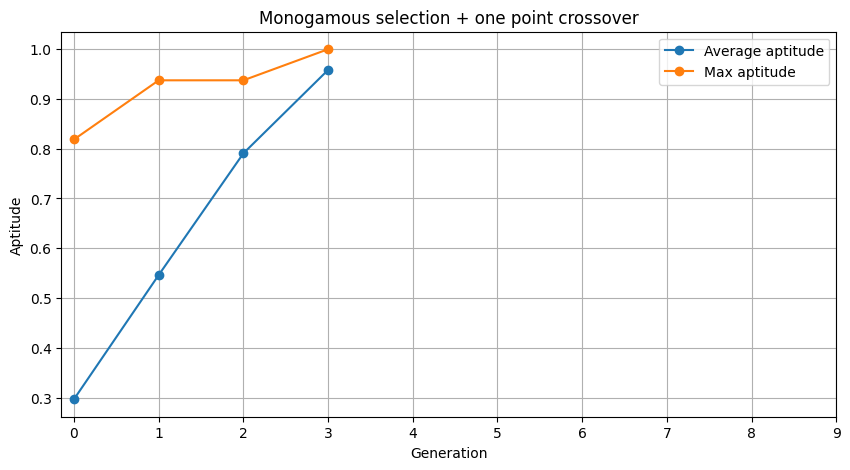
\includegraphics[width=0.4\textwidth]{monogamous_selection_one_point_crossover}
	\caption{Evolución de la aptitud de los individuos del algoritmo 1.}
	\label{fig: m_op}
\end{figure}

Este algoritmo muestra un buen rendimiento en términos de aptitud promedio y mejor aptitud, ya que logra una aptitud promedio alta y alcanza la mejor aptitud posible de $1$. Sin embargo, se requirieron 3 generaciones para llegar a este punto. Es posible que el algoritmo haya tenido que explorar varias soluciones antes de converger a la solución óptima.

Respecto al desempeño del algoritmo 2. Se tomó un total de $2$ generaciones en alcanzar el criterio de paro por épsilon, presentando una aptitud promedio final de $0.8434$ y teniendo a su mejor individuo con aptitud de $1.0000$. Este proceso de evolución se puede observar en la Figura \ref{fig: m_tp}.

\begin{figure}[htbp]
	\centering
	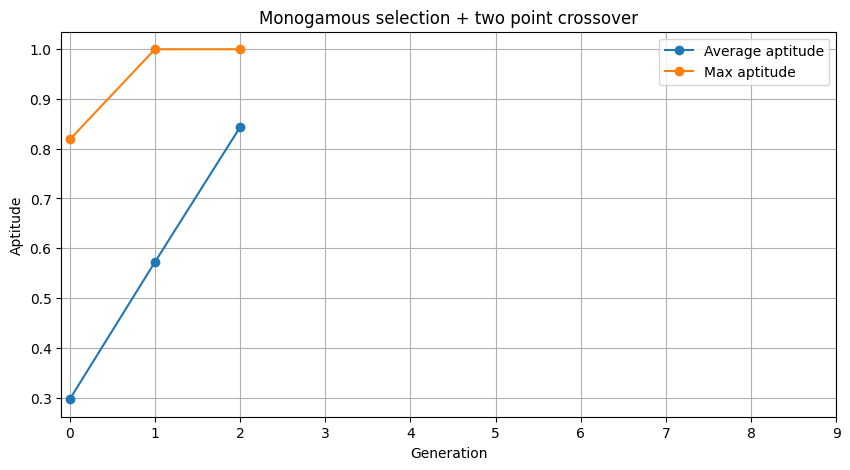
\includegraphics[width=0.4\textwidth]{monogamous_selection_two_point_crossover}
	\caption{Evolución de la aptitud de los individuos del algoritmo 2.}
	\label{fig: m_tp}
\end{figure}

En este caso, también presenta una alta mejor aptitud de $1$, pero en comparación con el Algoritmo 1, requiere solo $2$ generaciones. Aunque el valor promedio de aptitud es menor que el del Algoritmo 1, la rápida convergencia en solo $2$ generaciones es una característica destacable.

En cuanto al algoritmo 3. Este tardó un total de $5$ generaciones en alcanzar el paro por épsilon, logrando obtener una aptitud promedio final de $0.8219$, y teniendo a su mejor individuo con una aptitud de $1.0000$. Para este algoritmo podemos observar en la Figura \ref{fig: p_op} su proceso de evolución.

\begin{figure}[htbp]
	\centering
	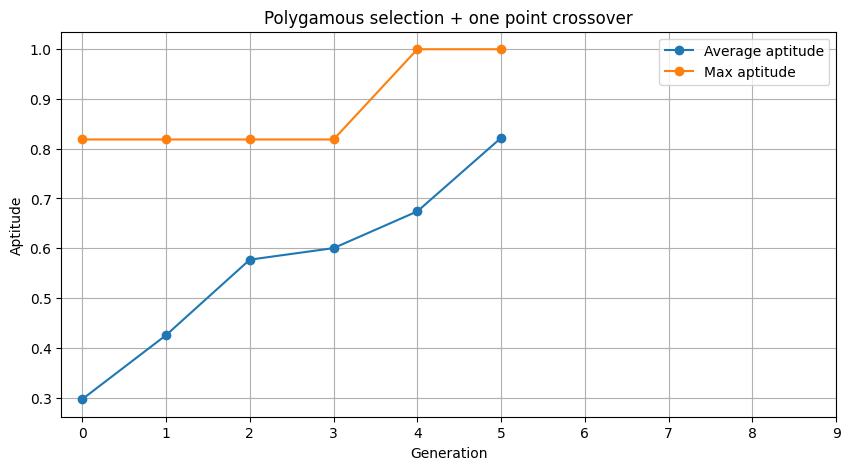
\includegraphics[width=0.4\textwidth]{polygamous_selection_one_point_crossover}
	\caption{Evolución de la aptitud de los individuos del algoritmo 3.}
	\label{fig: p_op}
\end{figure}

Dicho algoritmo tiene un mayor número de generaciones en comparación con los dos algoritmos anteriores. Aunque la aptitud promedio y la mejor aptitud siguen siendo altas, el mayor número de generaciones podría indicar que este algoritmo requiere más tiempo para converger hacia soluciones óptimas.

Por último, relacionado al algoritmo 4. Se tomo un total de $2$ generaciones en alcanzar el paro por épsilon, donde se obtuvo una aptitud promedio final de $0.8185$, y un mejor individuo con un valor igual de aptitud. El proceso de evolución de este algoritmo se puede observa en la Figura \ref{fig: p_tp}.

\begin{figure}[htbp]
	\centering
	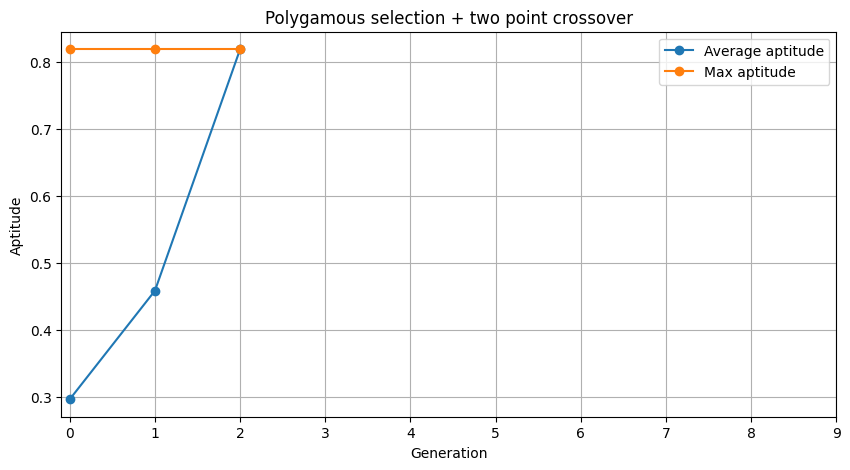
\includegraphics[width=0.4\textwidth]{polygamous_selection_two_point_crossover}
	\caption{Evolución de la aptitud de los individuos del algoritmo 4.}
	\label{fig: p_tp}
\end{figure}

Es importante notar que la mejor aptitud de este algoritmo no alcanza el valor máximo posible de $1$. Aunque este algoritmo requiere solo $2$ generaciones, su incapacidad para alcanzar la mejor aptitud posible podría indicar que está quedando atrapado en un óptimo local o necesita ajustes en su configuración.

\section{Conclusiones}
El objetivo principal de este trabajo, encontrar el precio optimo de los productos lacteos, se consiguió de forma satisfactoria. Es cierto que este ejercicio se realizó en gran parte con datos sintéticos, pero la implementación de este se deja abierta para el uso de datos reales del mercado y la industria específica.

Nuevamente se ha observado como los algoritmos genéticos son una herramienta muy valiosa para optimizar procesos en tiempos muy cortos, donde si utilizamos una codificación y función de aptitud adecuada podemos llegar a resultados óptimos.

Para el caso específico del análisis de datos, se puede destacar que siempre es necesario realizar análisis de diversas formas, ya que un análisis básico no siempre nos puede dar la información correcta. En este caso el primer análisis nos indicaba que la variación de precio era mínima, pero al corroborar con análisis más detallados se observó que en realidad no existe un precio que permanezca constante a lo largo del tiempo.



\nocite{*}
\renewcommand{\refname}{Referencias bibliográficas}
\bibliographystyle{IEEEtran-spanish}
\bibliography{referencias}

\end{document}